\documentclass[hyperref={pdfpagelabels=false},ngerman]{beamer}

\usepackage[T1]{fontenc}
\usepackage[utf8]{inputenc}
\usepackage[english]{babel}
\usepackage{lmodern}
\usepackage{graphicx}
\usepackage{amsmath,amssymb,amstext,amsfonts} % mathrsfs
% \usepackage{physics}
\usepackage{booktabs,tabularx}
\usepackage{tikz}
\usetikzlibrary{shapes,calc,arrows,positioning}
\tikzstyle{block} = [rectangle, draw, text width=10em, text centered, minimum height=2em]
\tikzstyle{arrow} = [draw, -latex, thick]
\usepackage{pgfplots}
\pgfplotsset{compat=1.18}
\usepgfplotslibrary{fillbetween,groupplots}
% \usepackage{multirow}
\usepackage{tcolorbox}
\usepackage{pifont}
\usepackage{xspace}
\usepackage{hyperref}
\hypersetup{colorlinks,linkcolor=,urlcolor=blue}

\definecolor{darkgreen}{RGB}{0,176,0}
\definecolor{darkred}{RGB}{200,0,0}
\definecolor{darkyellow}{RGB}{255,165,0}

\newcommand{\cmark}{\ding{51}}%
\newcommand{\xmark}{\ding{55}}%
\newcommand{\fmfvcenter}[1]{\;\vcenter{\hbox{\fmfreuse{#1}}}\;}
\newcommand{\eh}[1]{\,\mathsf{#1}}
\newcommand{\ok}{\textcolor{darkgreen}{\cmark}}
\newcommand{\notok}{\textcolor{red}{\xmark}}
\newcommand{\maybe}{\textcolor{gray}{\cmark}}
\newcommand{\meh}{\textcolor{gray}{\textbf{\huge\lower.1em\hbox{-}}}}
\newcommand{\Lagr}{\mathcal{L}}
\newcommand{\MS}{\ensuremath{M_S}}
\newcommand{\mathi}{\mathsf{i}}
\newcommand{\mycite}[1]{\ensuremath{\text{\textcolor{darkgray}{\tiny [#1]}}}}
\newcommand{\bigcite}[1]{\textcolor{darkgray}{[#1]}}
\newcommand{\dimrep}[1]{\mathbf{#1}}
\newcommand{\dimrepadj}[1]{\mathbf{\overline{#1}}}
\newcommand{\ESSM}{E\textsubscript{6}SSM}
\newcommand{\CESSM}{CE\textsubscript{6}SSM}
\renewcommand{\emph}[1]{\textbf{\textcolor{darkblue}{#1}}}
\newcommand{\myurl}[1]{\href{#1}{#1}}
\newcommand{\Superpot}{\mathcal{W}}
\newcommand{\SuperField}[1]{#1}
\newcommand{\ConjSuperField}[1]{\bar{#1}}
\newcommand{\UY}{\ensuremath{U(1)_{Y}}}
\newcommand{\UN}{\ensuremath{U(1)_{N}}}
\newcommand{\Uem}{\ensuremath{U(1)_\text{em}}}
\newcommand{\SUL}{\ensuremath{SU(2)_\text{L}}}
\newcommand{\SUc}{\ensuremath{SU(3)_\text{c}}}
\newcommand{\SOten}{\ensuremath{{SO(10)}}}
\newcommand{\comma}{,}
\newcommand{\DRbar}{\ensuremath{\overline{\text{DR}}}}
\newcommand{\DRbarp}{\ensuremath{\overline{\text{DR}}'}}
\newcommand{\MSbar}{\ensuremath{\overline{\text{MS}}}}
\newcommand{\SM}{\ensuremath{\text{SM}}}
\newcommand{\MSSM}{\ensuremath{\text{MSSM}}}
\newcommand{\BSM}{\ensuremath{\text{BSM}}}
\newcommand{\EFT}{\ensuremath{\text{EFT}}\xspace}
\newcommand{\THDM}{\ensuremath{\text{2HDM}}\xspace}
\newcommand{\pole}{\ensuremath{\text{pole}}}
\newcommand{\tree}{\ensuremath{\text{tree}}}
\newcommand{\fsstar}{\textbf{*}}
\newcommand{\FS}{\texttt{FlexibleSUSY}\xspace}
\newcommand{\fsh}{\texttt{FS+H}\xspace}
\newcommand{\feft}{\texttt{FlexibleEFTHiggs}\xspace}
\newcommand{\hssusy}{\texttt{HSSUSY}\xspace}
\newcommand{\Himalaya}{\texttt{Himalaya}\xspace}
\newcommand{\FH}{\texttt{FeynHiggs}\xspace}
\newcommand{\SPheno}{\texttt{SPheno}\xspace}
\newcommand{\SARAH}{\texttt{SARAH}\xspace}
\newcommand{\SOFTSUSY}{\texttt{SOFTSUSY}\xspace}
\newcommand{\Zv}{\ensuremath{\backslash\mkern-11.0mu{Z_3}}}
\newcommand{\downrightknickarrow}{\mathrel{\scalebox{1.3}{\rotatebox[origin=c]{180}{$\Lsh$}}}}
\newcommand{\threelinebrace}{$\left. \begin{array}{c} \\ \\ \\ \end{array} \right\rbrace$}
\newcommand{\fivelinebrace}{$\left. \begin{array}{c} \\ \\ \\ \\ \\ \end{array} \right\rbrace$}
\newcommand{\twolinebrace}{$\left. \begin{array}{c} \\ \\ \end{array} \right\rbrace$}
\newcommand{\elevenlinebrace}{$\left. \begin{array}{c} \\ \\ \\ \\ \\ \\ \\ \\ \\ \\ \\ \end{array} \right\rbrace$}
\newcommand{\at}{\alpha_t}
\newcommand{\ab}{\alpha_b}
\newcommand{\atau}{\alpha_\tau}
\newcommand{\as}{\alpha_s}
\newcommand{\aem}{\alpha_\text{em}}
\newcommand{\GeV}{\eh{GeV}}
\newcommand{\TeV}{\eh{TeV}}
\newcommand{\SQCD}{\ensuremath{\scalefont{.8}\text{SQCD}}}
\newcommand{\Qpole}{\ensuremath{Q_\text{pole}}}
\newcommand{\Qlow}{\ensuremath{Q_\text{low}}}
\newcommand{\Qmatch}{\ensuremath{Q_\text{match}}}
\newcommand{\Qsplit}{\ensuremath{Q_\text{split}}\xspace}
\newcommand{\QTHDM}{\ensuremath{Q_\text{\THDM}}\xspace}
\newcommand{\DMh}{\ensuremath{\Delta M_h^{(\texttt{SS+H})}}}
\newcommand{\DMhQpole}{\ensuremath{\Delta M_h^{(\Qpole)}}}
\newcommand{\DMhQmatch}{\ensuremath{\Delta M_h^{(\Qmatch)}}}
\newcommand{\DMhMt}{\ensuremath{\Delta M_h^{(m_t)}}}
\newcommand{\DMhAlphaS}{\ensuremath{\Delta M_h^{(\as)}}}
\newcommand{\DMhAlphaEm}{\ensuremath{\Delta M_h^{(\aem)}}}
\newcommand{\DMhHSSUSY}{\ensuremath{\Delta M_h^{(\HSSUSY)}}}
\newcommand{\DMhHSSUSYytSM}{\ensuremath{\Delta M_h^{(\hat{y}_t)}}}
\newcommand{\DMhHSSUSYytMSSM}{\ensuremath{\Delta M_h^{(y_t^\MSSM)}}}
\newcommand{\DMhEFT}{\ensuremath{\Delta M_h^{(v^2/\MS^2)}}}
\newcommand{\Mathematica}{\texttt{Mathematica}}
\newcommand{\Loop}{\ensuremath{\ell}}
\newcommand{\ord}{\ensuremath{\mathcal{O}}}
\def\HSSUSY{\texttt{HSSUSY}}

% set look of slides
\usetheme{Madrid}
\useoutertheme{default}
\useinnertheme{circles}
\usecolortheme{default}
\beamertemplatenavigationsymbolsempty % keine Navigationselemente
\setbeamersize{text margin left = 1cm, text margin right = 1cm}

% define footer
\makeatletter
\setbeamertemplate{footline}
{
  \hfill\hbox{\insertframenumber{} / \inserttotalframenumber\hspace*{4pt}}%
  \vskip3pt%
}
\makeatother
\usecolortheme{tud}

\title{Status of the $M_h$ prediction in the MSSM with FlexibleSUSY}

\author[Alexander Voigt]{Alexander Voigt}

\date{pMSSM topic meeting\\[1em] March 2nd 2026}

% \institute[Aachen]{RWTH Aachen}
\subject{MSSM,Higgs,Supersymmetrie,EFT}
\keywords{MSSM,Higgs,Supersymmetrie,EFT}

%%%%%%%%%%%%%%%%%%%%%%%%%%%%%%%%%%%%%%%%%%%%%%%%%%%%%%%%%%%%%%%%%%%%%%%%%%%%%

\begin{document}

%%%%%%%%%%%%%%%%%%%%%%%%%%%%%%%%%%%%%%%%

\begin{frame}[plain]
  \begin{tikzpicture}[remember picture,overlay]
    \node[anchor=south east] at ([yshift=0.5cm,xshift=-0.5cm]current page.south east) {\includegraphics[width=4cm]{images/RWTH_Logo.pdf}};
    \node[anchor=south west] at ([yshift=0.5cm,xshift=0.5cm]current page.south west) {\includegraphics[width=4cm]{images/FS-logo.png}};
  \end{tikzpicture}
  \titlepage
\end{frame}

%%%%%%%%%%%%%%%%%%%%%%%%%%%%%%%%%%%%%%%%

\begin{frame}{Contents}
  \tableofcontents
\end{frame}

%%%%%%%%%%%%%%%%%%%%%%%%%%%%%%%%%%%%%%%%

\section{Fixed-order calculation}

%%%%%%%%%%%%%%%%%%%%%%%%%%%%%%%%%%%%%%%%%%%%%%%%%%%%%%%%%%%%

\begin{frame}{Contents}
  \tableofcontents[currentsection,currentsubsection]
\end{frame}

%%%%%%%%%%%%%%%%%%%%%%%%%%%%%%%%%%%%%%%%%%%%%%%%%%%%%%%%%%%%

\begin{frame}{Fixed-order calculation (\texttt{NUHMSSMNoFVHimalaya})}
  \emph{Input:} $\aem(M_Z)$, $\as(M_Z)$, $G_F$, $M_Z$, $M_t$, $m_b(m_b)$,\\
  SUSY parameters ($m_{\tilde{f}}^2$, $A_f$, $M_i$, $\mu$, $B\mu$), \ldots
  %
  \begin{center}
    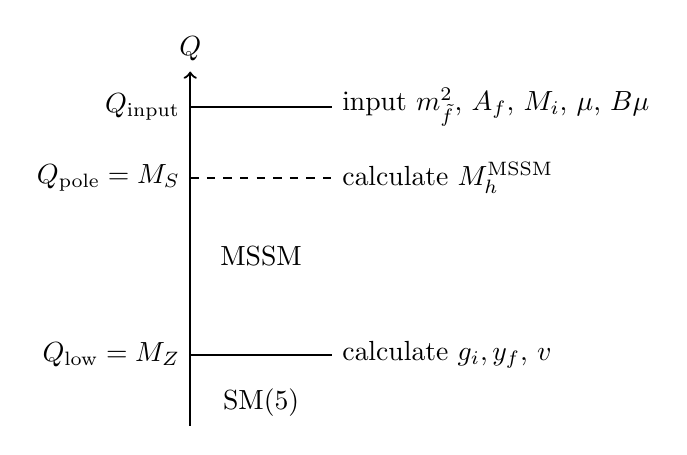
\begin{tikzpicture}[scale=0.9]
      \pgfmathsetmacro{\breite}{2};
      \draw[->, thick] (0,0) -- (0,5) node[above] {$Q$};
      \draw[thick] (0,4.5) node[left]{$Q_\text{input}$} -- ++ (\breite,0) node[right]{input $m_{\tilde{f}}^2$, $A_f$, $M_i$, $\mu$, $B\mu$};
      \draw[thick,dashed] (0,3.5) node[left]{$\Qpole=\MS$} -- ++ (\breite,0) node[right]{calculate $M_h^\MSSM$};
      \draw[thick] (0,1) node[left]{$\Qlow=M_Z$} -- node[above=1cm,black]{MSSM} node[below=0.3cm,black]{SM(5)} ++ (\breite,0) node[right]{calculate $g_i, y_f$, $v$};
    \end{tikzpicture}
  \end{center}
\end{frame}

%%%%%%%%%%%%%%%%%%%%%%%%%%%%%%%%%%%%%%%%%%%%%%%%%%

\begin{frame}{Precision of fixed-order calculation (\texttt{NUHMSSMNoFVHimalaya})}
  \begin{center}
    \begin{tabular}{llll}
      \toprule
      & 1\Loop & 2\Loop & 3\Loop\\
      \midrule
      $y_t$      & full & $y_tg_3^4$ & -- \\
      $y_{b,\tau}$ & full & -- & -- \\
      $g_3$      & full & $g_3^4$ & -- \\
      $g_{1,2}$   & full & -- & -- \\
      $v$        & full & -- & -- \\
      \midrule
      $\beta_{y_t}$    & full & full & full \\
      $\beta_{g_3}$    & full & full & full \\
      $\beta_{\ldots}$    & full & full & full \\
      $\beta_{v_i}$  & full & full & -- \\
      \midrule
      $M_h$  & full & $g_3^2(y_t^4+y_b^4)+(y_t^2+y_b^2)^3+(y_t^2+y_\tau^2)^3$ & $g_3^4 y_t^4$ \\
      \bottomrule
    \end{tabular}
  \end{center}
  % \textcolor{red}{red}: incomplete contributions w.r.t.\ $M_h$
\end{frame}

%%%%%%%%%%%%%%%%%%%%%%%%%%%%%%%%%%%%%%%%%%%%%%%%%%

\newcommand{\NUHMSSMNoFVHimalayaMSdata}{data/NUHMSSMNoFVHimalaya_MS-Mh-DMh_TB-20_xt--2.44949.dat}
\newcommand{\NUHMSSMNoFVHimalayaXtdata}{data/NUHMSSMNoFVHimalaya_Xt-Mh-DMh_MS-3000_TB-20.dat}

\begin{frame}{Uncertainty estimate of the fixed-order calculation}
  \begin{center}
    \begin{tikzpicture}
      \begin{groupplot}[
        group style={
          group size=1 by 2,
          vertical sep=0,
        },
        height={0.65\textheight},
        width={0.7\textwidth},
        xmode=log,
        log basis x=10,
        xmin=400, xmax=10000,
        grid
        ]
        \nextgroupplot[
          title={$\tan\beta=20$, $x_t=-\sqrt{6}$},
          ymin=110, ymax=135,
          ytick={115,120,125,130,135},
          ylabel={$M_h$ / GeV},
          xticklabels=\empty
        ]
        \addplot[red,thick] table[x index=0, y index=1] {\NUHMSSMNoFVHimalayaMSdata};
        \addplot[name path=upper,draw=none] table[x index=0, y expr=\thisrowno{1}+\thisrowno{2}] {\NUHMSSMNoFVHimalayaMSdata};
        \addplot[name path=lower,draw=none] table[x index=0, y expr=\thisrowno{1}-\thisrowno{2}] {\NUHMSSMNoFVHimalayaMSdata};
        \addplot[red!30,fill opacity=0.5] fill between[of=upper and lower];
        \nextgroupplot[height=3cm,ylabel={$\Delta M_h$ / GeV},xlabel={$\MS$ / GeV},ymin=0,ymax=4,ytick distance=1]
        \addplot[red,thick] table[x index=0,y index=2] {\NUHMSSMNoFVHimalayaMSdata};
      \end{groupplot}
    \end{tikzpicture}
  \end{center}
\end{frame}

%%%%%%%%%%%%%%%%%%%%%%%%%%%%%%%%%%%%%%%%%%%%%%%%%%

\begin{frame}{Uncertainty estimate of the fixed-order calculation}
  \begin{center}
    \begin{tikzpicture}
      \begin{groupplot}[
        group style={
          group size=1 by 2,
          vertical sep=0,
        },
        height={0.65\textheight},
        width={0.7\textwidth},
        xmin=-3.5, xmax=3.5,
        grid
        ]
        \nextgroupplot[
          title={$\MS=3$ TeV, $\tan\beta=20$},
          ymin=105,
          ymax=135,
          ytick={110,115,120,125,130,135},
          ylabel={$M_h$ / GeV},
          xticklabels=\empty
        ]
        \addplot[red,thick] table[x index=0, y index=1] {\NUHMSSMNoFVHimalayaXtdata};
        \addplot[name path=upper,draw=none] table[x index=0, y expr=\thisrowno{1}+\thisrowno{2}] {\NUHMSSMNoFVHimalayaXtdata};
        \addplot[name path=lower,draw=none] table[x index=0, y expr=\thisrowno{1}-\thisrowno{2}] {\NUHMSSMNoFVHimalayaXtdata};
        \addplot[red!30,fill opacity=0.5] fill between[of=upper and lower];
        \nextgroupplot[height=3cm,ylabel={$\Delta M_h$ / GeV},xlabel={$x_t$ },ymin=0,ymax=3,ytick distance=1]
        \addplot[red,thick] table[x index=0,y index=2] {\NUHMSSMNoFVHimalayaXtdata};
      \end{groupplot}
    \end{tikzpicture}

  \end{center}
\end{frame}

%%%%%%%%%%%%%%%%%%%%%%%%%%%%%%%%%%%%%%%%

\section{Pure Effective Field Theory}

\begin{frame}{Contents}
  \tableofcontents[currentsection,currentsubsection]
\end{frame}

\begin{frame}{Pure EFT calculation (\texttt{HSSUSY})}
  \emph{Input:} same as in fixed-order calculation
  \begin{center}
  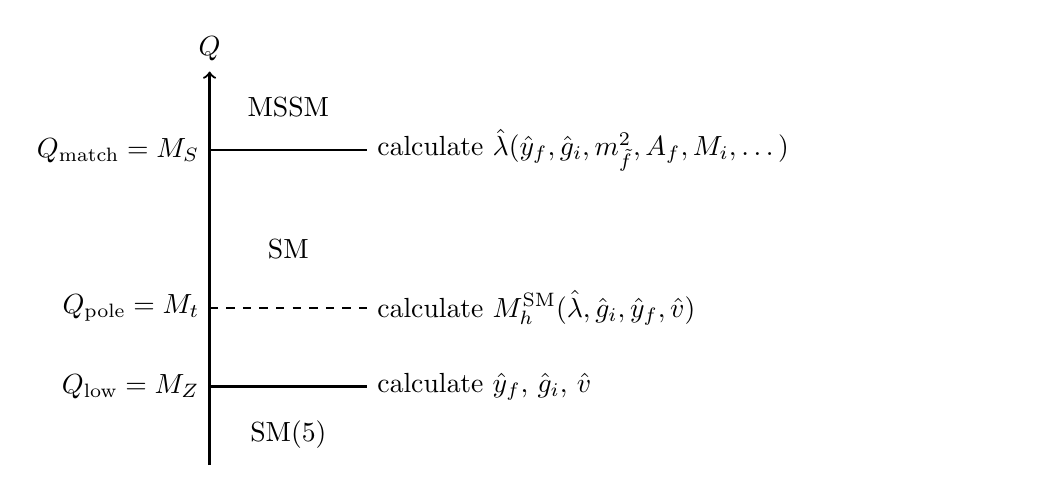
\begin{tikzpicture}
    \pgfmathsetmacro{\breite}{2};
    \draw[->,thick] (0,0) -- (0,5) node[above]{$Q$};
    \draw[thick] (0,4) node[left]{$\Qmatch = \MS$} -- node[above = 0.3cm,black]{MSSM} (\breite,4) node[right,black]{calculate $\hat\lambda(\hat y_f, \hat g_i, m_{\tilde{f}}^2, A_f, M_i,\dotsc)$};
    \draw[thick,dashed] (0,2) node[left]{$\Qpole = M_t$} -- (\breite,2) node[right,black,text width=8cm]{calculate $M_h^\SM(\hat\lambda, \hat g_i, \hat y_f, \hat v)$};
    \draw[thick] (0,1) node[left]{$\Qlow = M_Z$} -- node[above = 1.5cm,black]{SM} node[below = 0.3cm,black]{SM(5)} (\breite,1) node[right,black,text width=8cm]{
      calculate $\hat y_f$, $\hat g_i$, $\hat v$};
    % \draw[<->,blue,thick] (-2.5,1) -- node[above,rotate=90]{RG running} (-2.5,4);
  \end{tikzpicture}
  \end{center}
\end{frame}

%%%%%%%%%%%%%%%%%%%%%%%%%%%%%%%%%%%%%%%%%%%%%%%%%%

\begin{frame}{Pure EFT calculation (\texttt{HSSUSY})}
  \begin{center}
    \begin{tabular}{llllll}
      \toprule
      & 1\Loop & 2\Loop & 3\Loop & 4\Loop & 5\Loop\\
      \midrule
      $\hat\lambda$  & full & $(\hat{y}_t^4+\hat{y}_b^4)\hat{g}_3^2+(\hat{y}_t^4+\hat{y}_b^4+\hat{y}_\tau^4)^2$ & $\hat{y}_t^4\hat{g}_3^4$ & -- & -- \\
      $\hat{v}$        & full & -- & -- & -- & -- \\
      $\hat{y}_t$      & full & $\hat{y}_t\hat{g}_3^4\textcolor{gray}{\,+\,\hat{y}_t^3 \hat{g}_3^2+\hat{y}_t^5}$ & \textcolor{gray}{$\hat{y}_t\hat{g}_3^6$} & $\textcolor{gray}{\hat{y}_t\hat{g}_3^8}$ & -- \\
      $\hat{y}_{b,\tau}$ & full & -- & -- & -- & -- \\
      $\hat{g}_3$      & full & $\hat{g}_3^4$ &  $\hat{g}_3^6$ & -- & -- \\
      $\hat{g}_{1,2}$   & full & -- & -- & -- & -- \\
      \midrule
      $\beta_{\hat\lambda}$ & full & full & full & $\hat{y}_t^4\hat{g}_3^6$ & -- \\
      $\beta_{\hat{y}_t}$    & full & full & full & $\hat{y}_t\hat{g}_3^8$ & -- \\
      $\beta_{\hat{g}_3}$    & full & full & full & $\hat{g}_3^{0<n\le 8}$ & $\hat{g}_3^{10}$ \\
      $\beta_{\cdots}$  & full & full & full & -- & -- \\
      \midrule
      $M_h$           & full & $(\hat{y}_t^4+\hat{y}_b^4)\hat{g}_3^2+(\hat{y}_t^4 + \hat{y}_b^4)^2$ & $\hat{y}_t^4 \hat{g}_3^4\textcolor{gray}{\,+\,\hat{y}_t^6\hat{g}_3^2+\hat{y}_t^8}$ & \textcolor{gray}{$\hat{y}_t^4 \hat{g}_3^6$} & -- \\
      \bottomrule
    \end{tabular}
  \end{center}
  \textcolor{gray}{gray}: incomplete contributions w.r.t.\ $M_h$
\end{frame}

%%%%%%%%%%%%%%%%%%%%%%%%%%%%%%%%%%%%%%%%%%%%%%%%%%

\begin{frame}{Uncertainty estimate of the EFT calculation}
  Sources of uncertainty:
  \begin{align*}
    \DMhQpole &= \max_{\Qpole\in[M_t/2,2M_t]}\left|M_h(\Qpole) - M_h(M_t)\right| & \text{\mycite{1609.00371}} \\
    \DMhQmatch &= \max_{\Qmatch\in[\MS/2,2\MS]}\left|M_h(\Qmatch) - M_h(\MS)\right| & \text{\mycite{1407.4081}} \\
    \DMhHSSUSYytSM &= \left| M_h(\hat{y}_t^{3\Loop}(M_Z)) - M_h(\hat{y}_t^{4\Loop}(M_Z)) \right| & \text{\mycite{1504.05200}} \\
    \DMhEFT &= \left| M_h - M_h(v^2/\MS^2) \right| & \text{\mycite{1504.05200}} % \\
    % \DMhHSSUSYytMSSM &= \left| M_h - M_h(y_t^\MSSM(\MS)) \right| & \text{\mycite{Bagnaschi,AV,Weiglein}}
  \end{align*}
  Combination:
  \begin{equation*}
    \DMhHSSUSY = \DMhQpole + \DMhQmatch + \DMhHSSUSYytSM % + \DMhHSSUSYytMSSM \\
    + \DMhEFT
  \end{equation*}
\end{frame}

%%%%%%%%%%%%%%%%%%%%%%%%%%%%%%%%%%%%%%%%%%%%%%%%%%

\newcommand{\HSSUSYMSdata}{data/HSSUSY_MS-Mh-DMh_TB-20_xt--2.44949.dat}
\newcommand{\HSSUSYXtdata}{data/HSSUSY_Xt-Mh-DMh_MS-3000_TB-20.dat}

\begin{frame}{Uncertainty estimate of the EFT calculation}
  \begin{center}
    \begin{tikzpicture}
      \begin{groupplot}[
        group style={
          group size=1 by 2,
          vertical sep=0,
        },
        height={0.65\textheight},
        width={0.7\textwidth},
        xmode=log,
        log basis x=10,
        xmin=400, xmax=10000,
        grid
        ]
        \nextgroupplot[
          title={$\tan\beta=20$, $x_t=-\sqrt{6}$},
          ymin=110, ymax=130,
          ytick={115,120,125,130},
          ylabel={$M_h$ / GeV},
          xticklabels=\empty
        ]
        \addplot[red,thick] table[x index=0, y index=1] {\HSSUSYMSdata};
        \addplot[name path=upper,draw=none] table[x index=0, y expr=\thisrowno{1}+\thisrowno{2}] {\HSSUSYMSdata};
        \addplot[name path=lower,draw=none] table[x index=0, y expr=\thisrowno{1}-\thisrowno{2}] {\HSSUSYMSdata};
        \addplot[red!30,fill opacity=0.5] fill between[of=upper and lower];
        \nextgroupplot[height=3cm,ylabel={$\Delta M_h$ / GeV},xlabel={$\MS$ / GeV},ymin=0,ymax=4,ytick distance=1]
        \addplot[red,thick] table[x index=0,y index=2] {\HSSUSYMSdata};
      \end{groupplot}
    \end{tikzpicture}
  \end{center}
\end{frame}

%%%%%%%%%%%%%%%%%%%%%%%%%%%%%%%%%%%%%%%%%%%%%%%%%%

\begin{frame}{Uncertainty estimate of the EFT calculation}
  \begin{center}
    \begin{tikzpicture}
      \begin{groupplot}[
        group style={
          group size=1 by 2,
          vertical sep=0,
        },
        height={0.65\textheight},
        width={0.7\textwidth},
        xmin=-3.5, xmax=3.5,
        grid
        ]
        \nextgroupplot[
          title={$\MS=3$ TeV, $\tan\beta=20$},
          ymin=105,
          ymax=130,
          ytick={110,115,120,125,130},
          ylabel={$M_h$ / GeV},
          xticklabels=\empty
        ]
        \addplot[red,thick] table[x index=0, y index=1] {\HSSUSYXtdata};
        \addplot[name path=upper,draw=none] table[x index=0, y expr=\thisrowno{1}+\thisrowno{2}] {\HSSUSYXtdata};
        \addplot[name path=lower,draw=none] table[x index=0, y expr=\thisrowno{1}-\thisrowno{2}] {\HSSUSYXtdata};
        \addplot[red!30,fill opacity=0.5] fill between[of=upper and lower];
        \nextgroupplot[height=3cm,ylabel={$\Delta M_h$ / GeV},xlabel={$x_t$ },ymin=0,ymax=2,ytick distance=1]
        \addplot[red,thick] table[x index=0,y index=2] {\HSSUSYXtdata};
      \end{groupplot}
    \end{tikzpicture}

  \end{center}
\end{frame}

%%%%%%%%%%%%%%%%%%%%%%%%%%%%%%%%%%%%%%%%

\section{Hybrid}

\begin{frame}{Contents}
  \tableofcontents[currentsection,currentsubsection]
\end{frame}

%%%%%%%%%%%%%%%%%%%%%%%%%%%%%%%%%%%%%%%%

% \begin{frame}{Comparison of fixed-order and EFT calculation}
%   \begin{center}
%     \includegraphics[width=0.49\textwidth]{plots/SOFTSUSY/Mh_MS_TB-20_Xt--sqrt6}\hfill
%     \includegraphics[width=0.49\textwidth]{plots/SOFTSUSY/HSSUSY_TB-20_Xt--sqrt6_individual}
%   \end{center}
%   \begin{center}
%     $\DMhFO \overset{!}{=} \DMhEFT$\\[0.5em]
%     $\Rightarrow$ $\MS^{\text{equal}} \sim 1\TeV$ for
%     small/large $\tan\beta$ and/or $X_t$
%   \end{center}
%   \mycite{1804.09410}
% \end{frame}

% \begin{frame}{Summary of fixed-order and EFT approaches}
%   \begin{center}
%     \begin{tabular}{lcc}
%       \toprule
%                   & low $\MS$ & high $\MS$ \\
%                   & $\MS \lesssim 1\eh{TeV}$ & $\MS \gtrsim 1\eh{TeV}$ \\
%       \midrule
%       fixed-order & \ok       & \notok     \\
%       EFT         & \notok    & \ok        \\
%       ? hybrid    & \ok       & \ok        \\
%       \bottomrule
%     \end{tabular}
%   \end{center}
%   \vspace{2em}
%   Q: Can the fixed-order and EFT approaches be combined? \\[1em]
%   A: Yes!  \mycite{1312.4937, 1609.00371, 1710.03760, 1910.03595, 2003.04639}
% \end{frame}

% %%%%%%%%%%%%%%%%%%%%%%%%%%%%%%%%%%%%%%%%

% \subsection{Hybrid}

% \begin{frame}{Contents}
%   \tableofcontents[currentsection,currentsubsection]  
% \end{frame}

% \begin{frame}{Hybrid calculation -- FeynHiggs approach}
%   \emph{Goal:} resum large logarithms \emph{and} include suppressed
%   $\ord(v^2/\MS^2)$ terms
%   \\[2em]
%   \emph{Idea I:} (``FeynHiggs approach'' \mycite{1312.4937, 1706.00346, 1805.00867, 1910.03595})\\
%   Replace logs from fixed-order calculation by resummed logs:
%   \begin{align*}
%     M_h^2 = (M_h^2)_{\text{fixed-order}} - (M_h^2)_{\text{logs}} + (M_h^2)_{\text{resummed logs}}
%   \end{align*}
%   \emph{Advantages:}
%   \begin{itemize}
%   \item[\ok] approach applicable to any BSM model
%   \item[\ok] any EFT can be used
%   \end{itemize}
%   \emph{Disadvantages:}
%   \begin{itemize}
%   \item[\notok] requires knowledge of fixed-order and EFT expressions
%   \item[\notok] care must be taken to avoid double counting
%   \end{itemize}
% \end{frame}

% \begin{frame}{FeynHiggs approach in FlexibleSUSY at 3-loop}
%   \begin{center}
%     \includegraphics[width=0.49\textwidth]{plots/Mh3l-match-really/scan_Mh_MS_TB-20_Xt--sqrt6_mixed_3L}\hfill
%     \includegraphics[width=0.49\textwidth]{plots/Mh3l-match-really/scan_Mh_MS_TB-20_Xt--sqrt6_mixed_3L_diff}
%   \end{center}
%   \mycite{1910.03595}
% \end{frame}

% \begin{frame}{Hybrid calculation -- FlexibleEFTHiggs}
%   % \emph{Goal:} resum large logarithms \emph{and} include suppressed
%   % $\ord(v^2/\MS^2)$ terms
%   % \\[2em]
%   \emph{Idea II:} (``FlexibleEFTHiggs'' \mycite{1609.00371,
%     1710.03760, 2003.04639})\\
%   Incorporate all $\ord((v^2/\MS^2)^\infty)$ terms into $\lambda$ by
%   using the matching condition for the FO calculations:
%   \begin{align*}
%     (M_h^2)_{\SM} &\overset{!}{=} (M_h^2)_{\BSM} \qquad \text{at } Q = \MS \\
%     \lambda(\MS) v^2 + (\Delta m_h^2)_{\SM} &= (M_h^2)_{\BSM}
%   \end{align*}
%   $\Rightarrow$
%   \begin{align*}
%     \lambda(\MS) = \frac{1}{v^2}\left[(M_h^2)_{\BSM} - (\Delta m_h^2)_{\SM}\right]
%   \end{align*}
%   Continue as in the EFT calculation \ldots
%   % \emph{Pro:}
%   % \begin{itemize}
%   % \item[\ok] approach applicable to any BSM model
%   %   % easy to apply to any SM extensison
%   % \item[\ok] easy to automate
%   %   (only fixed-order expressions required)
%   % \end{itemize}
%   % \emph{Contra:}
%   % \begin{itemize}
%   % \item[\notok] difficult to extend to other EFTs beyond the SM (2HDM,
%   %   \ldots)
%   % \item[\meh] tricky to reach 2-loop accuracy\\
%   %   (requires careful treatment of parameter matching)
%   % \end{itemize}
% \end{frame}

% \begin{frame}{Hybrid calculation -- FlexibleEFTHiggs}
%   Continue as in the EFT calculation:
%   \begin{center}
%     \begin{tikzpicture}[scale=0.9]
%       \draw[->, thick] (0,0) -- (0,1) node[left]{$M_t$} -- (0,5) node[left]{$\MS$} -- (0,6);
%       \draw[thick] (1,0)   rectangle node{SM(5)} (4,0.9);
%       \draw[thick] (1,1.1) rectangle node{SM}    (4,4.9);
%       \draw[thick] (1,5.1) rectangle node{BSM}  (4,6);
%       \draw[<-, thick, darkgreen] (4.1,5) -- (4.5,5) node[right]{$\lambda(\MS) = \frac{1}{v^2}\left[(M_h^2)_{\BSM} - (\Delta m_h^2)_{\SM}\right]$};
%       \draw[<-, thick, red] (4.1,1) -- (4.5,1) node[right]{$(M_h^\SM)^2 = \lambda(M_t) v^2 + (\Delta m_h^2)_{\SM} + \cdots$};
%       \draw[<->, thick, blue] (4.2,1.2) -- node[right]{RG running} (4.2,4.8);
%     \end{tikzpicture}
%   \end{center}
% \end{frame}

% %%%%%%%%%%%%%%%%%%%%%%%%%%%%%%%%%%%%%%%%

% \begin{frame}{Proof: FlexibleEFTHiggs $\rightarrow$ EFT for $v^2 \ll M_S^2$}
%   Consider the matching condition:
%   \begin{align*}
%     \lambda(\MS) = \frac{1}{v^2}\left[(M_h^2)_{\MSSM} - (\Delta m_h^2)_{\SM}\right]
%   \end{align*}
%   where at $\ord(y_t^4)$:
%   \begin{align*}
%     (\Delta m_h^2)_{\SM} ={}& - {\color{red}\Sigma^{\SM}_h} - {\color{red}6\kappa y_t^2 A_0(m_t)}\\
%     (M_h^2)_{\MSSM} ={}& m_Z^2 c^2_{2\alpha} + \Big[ - {\color{red}\Sigma_h^\SM}
%       - {\color{red} 6 \kappa y_t^2 A_0(m_t)} \Big] \; \frac{c^2_\alpha}{s^2_\beta} \\
%     &- 6 \kappa y_t^4 v^2 \frac{c^2_\alpha}{s^2_\beta} B_0(\MS,\MS)
%   \end{align*}
% \end{frame}

% \begin{frame}{Proof: FlexibleEFTHiggs $\rightarrow$ EFT for $v^2 \ll M_S^2$}
%   \begin{align*}
%     \lambda(\MS) ={}& \frac{1}{v^2}\left[(M_h^2)_{\MSSM} - (\Delta m_h^2)_{\SM}\right] \\
%     ={}& \frac{m_Z^2}{v^2} c^2_{2\alpha}
%     + \frac{1}{v^2} \Big[ - {\color{red}\Sigma_h^\SM}
%     - {\color{red} 6 \kappa y_t^2 A_0(m_t)} \Big] \; \Big(\frac{c^2_\alpha}{s^2_\beta} - 1 \Big) \\
%     &- 6 \kappa y_t^4 \frac{c^2_\alpha}{s^2_\beta} B_0(\MS,\MS)
%   \end{align*}
%   In the limit $v^2 \ll M_S^2$: $c_\alpha^2 \to s_\beta^2$, $c_{2\alpha}^2 \rightarrow c_{2\beta}^2$
%   $\Rightarrow$
%   \begin{align*}
%     \lambda(\MS) ={}& \frac{1}{4} (g_Y^2 + g_2^2) c_{2\beta}^2
%     - 6 \kappa y_t^4 B_0(\MS,\MS) \\
%     ={}& \frac{1}{4} (g_Y^2 + g_2^2) c_{2\beta}^2
%     - 6 \kappa y_t^4 \Big[
%     - \log\frac{\MS^2}{Q^2} + \textcolor{blue}{\frac{p^2}{6 \MS^2} + \ord\Big(\frac{p^4}{\MS^4}\Big)} \Big]
%   \end{align*}
% \end{frame}

% %%%%%%%%%%%%%%%%%%%%%%%%%%%%%%%%%%%%%%%%

% \begin{frame}{Summary of FlexibleEFTHiggs hybrid calculation}
%   Matching condition:
%   \begin{align*}
%     (M_h^2)_{\SM} &\overset{!}{=} (M_h^2)_{\BSM}
%   \end{align*}
%   \emph{Advantages:}
%   \begin{itemize}
%   \item[\ok] includes all power-suppressed terms at $n$-loop order
%     $(v^2/\MS^2)^\infty [c + \log^n(\MS/Q) + \log^n(\MS/m_t)]$
%   \item[\ok] resumms large non-suppressed logarithms $c \log^\infty(\MS/m_t)$
%   \item[\ok] approach applicable to any BSM model
%     % easy to apply to any SM extensison
%   \item[\ok] only 1- and 2-point fixed-order expressions required
%    $\rightarrow$ easy to automate (e.g.\ SARAH/FlexibleSUSY)
%   \end{itemize}
%   \emph{Disadvantages:}
%   \begin{itemize}
%   \item[\notok] difficult to extend to other EFTs beyond the SM (2HDM,
%     \ldots)
%   \item[\meh] tricky to reach 2-loop accuracy\\
%     (requires careful treatment of parameter matching)
%   \end{itemize}
% \end{frame}

% %%%%%%%%%%%%%%%%%%%%%%%%%%%%%%%%%%%%%%%%

% \begin{frame}{Interpolation behaviour of FlexibleEFTHiggs in the MSSM}
%   Interpolation behaviour between FO and EFT calculation:
%   \begin{center}
%     \includegraphics[width=0.49\textwidth]{{{plots/FlexibleEFTHiggs-2L/Mh_MS_TB-20_Xt-0}}}\hfill
%     \includegraphics[width=0.49\textwidth]{{{plots/FlexibleEFTHiggs-2L/Mh_MS_TB-20_Xt--sqrt6}}}
%   \end{center}
%   \begin{raggedright}
%     \mycite{plots along the lines of 2003.04639}
%   \end{raggedright}
% \end{frame}

% %%%%%%%%%%%%%%%%%%%%%%%%%%%%%%%%%%%%%%%%

% \begin{frame}{Hybrid calculation -- FlexibleEFTHiggs}
%   \begin{center}
%     \includegraphics[width=0.49\textwidth]{{{plots/FlexibleEFTHiggs-3L/uncer_2panel_ms_scan_xt-sqrt6_tb20}}}\hfill
%     \includegraphics[width=0.49\textwidth]{{{plots/FlexibleEFTHiggs-3L/uncer_2panel_xt_scan_ms3_tb20}}}
%   \end{center}
%   \begin{raggedright}
%     \mycite{2003.04639}
%   \end{raggedright}\\[1em]
%   Theory uncertainty $\DMh \lesssim 1\GeV$ in relevant degenerate SUSY scenarios.
% \end{frame}

% %%%%%%%%%%%%%%%%%%%%%%%%%%%%%%%%%%%%%%%%

% \section{$x_t$ resummation}
% \begin{frame}{Contents}
%   \tableofcontents[currentsection,currentsubsection]  
% \end{frame}

% \begin{frame}{Further improvements: $x_t$ resummation}
%   Large stop mixing, $x_t \equiv X_t/\MS \approx \pm \sqrt{6}$, is an
%   attractive scenario for low-scale supersymmetry.
%   \\[1em]
%   However: ``With large stop mixing comes large uncertainty.''\\
%   --- P.\ Slavich
%   \begin{center}
%     \includegraphics[width=0.49\textwidth]{{{plots/FlexibleEFTHiggs-1L/xt_MSSM_MS-2000}}}\hfill
%     \includegraphics[width=0.49\textwidth]{{{plots/1912.04199/var_XtDR}}}
%   \end{center}
%   \begin{raggedright}
%     \mycite{1609.00371, 1912.10002}
%   \end{raggedright}
% \end{frame}

% %%%%%%%%%%%%%%%%%%%%%%%%%%%%%%%%%%%%%%%%

% \begin{frame}{Recap: $\tan\beta$ resummation in $m_b$}
%   Relation between running $m_b$ in the MSSM and $m_b^{\EFT}$ in the EFT:
%   \begin{align*}
%     m_b^{\EFT} = m_b (1 + \Delta m_b)
%   \end{align*}
%   where $\Delta m_b$ is expressed in terms of MSSM parameters.\\[1em]
%   \begin{theorem}[hep-ph/9912516]
%     There are no contributions to $\Delta m_b$ of
%     $\ord((\as\tan\beta)^n)$ for $n\ge 2$.
%   \end{theorem}
%   \vspace*{1em}
%   $\Rightarrow$ All higher-order MSSM contributions in $m_b$ of
%   $\ord((\as\tan\beta)^n)$ can be resummed by writing:
%   \begin{align*}
%     m_b = \frac{m_b^{\EFT}}{1 + \Delta m_b}
%     = m_b^{\EFT} \sum_{n=0}^\infty (-\Delta m_b)^n
%   \end{align*}
% \end{frame}

% %%%%%%%%%%%%%%%%%%%%%%%%%%%%%%%%%%%%%%%%

% \begin{frame}{$x_t$ resummation}
%   Relation between running $y_t$ in the MSSM and $y_t^{\EFT}$ in the EFT:
%   \begin{align*}
%     y_t^{\EFT} = y_t s_\beta + \Delta y_t
%   \end{align*}
%   where $\Delta y_t$ is expressed in terms of MSSM parameters.\\[1em]
%   \begin{theorem}[Kwasnitza, Stöckinger (2003.04639)]
%     There are no unsuppressed contributions to $\Delta y_t$
%     of $\ord(\as^n x_t^{>1})$ for $n\ge 1$.
%   \end{theorem}
%   \vspace*{1em}
%   $\Rightarrow$ All higher-order MSSM contributions in $y_t$ of
%   $\ord(\as^n x_t^{>1})$ can be resummed by writing:
%   \begin{align*}
%     y_t = \frac{y_t^{\EFT}}{1 + \Delta y_t/(y_ts_\beta)}
%   \end{align*}
% \end{frame}

% %%%%%%%%%%%%%%%%%%%%%%%%%%%%%%%%%%%%%%%%

% % \begin{frame}{$x_t$ resummation}
% %   $\Rightarrow$ by expressing $M_h$ in terms of \emph{MSSM parameters}
% %   ($y_t$, $m_b$, \ldots), certain higher-order contributions can be
% %   resummed to all orders.
% %   \begin{center}
% %     \includegraphics[width=0.49\textwidth]{{{plots/FlexibleEFTHiggs-3L/plot_xt_MS_3_tb20_compare_hybrids}}}\hfill
% %     \includegraphics[width=0.49\textwidth]{{{plots/FlexibleEFTHiggs-3L/plot_xt_MS_3_tb20_compare_hybrids_diff}}}
% %   \end{center}
% %   \mycite{2003.04639}
% % \end{frame}

% \begin{frame}{$x_t$ resummation}
%   $\Rightarrow$ by expressing $\lambda(\MS)$ in terms of \emph{MSSM parameters}
%   ($y_t$, $m_b$, \ldots), certain higher-order contributions can be
%   resummed to all orders
%   \begin{center}
%     \includegraphics[width=0.49\textwidth]{{{plots/FlexibleEFTHiggs-3L/plot_MS_xt_sqrt6_tb20_compare_hybrids}}}\hfill
%     \includegraphics[width=0.49\textwidth]{{{plots/FlexibleEFTHiggs-3L/plot_MS_xt_sqrt6_tb20_compare_hybrids_diff}}}
%   \end{center}
%   \mycite{2003.04639}
% \end{frame}

% %%%%%%%%%%%%%%%%%%%%%%%%%%%%%%%%%%%%%%%%

% \section{Summary and conclusions}

% %%%%%%%%%%%%%%%%%%%%%%%%%%%%%%%%%%%%%%%%

% \begin{frame}{Summary and Conclusions}
%   \emph{Precise prediction of the Higgs boson mass} in supersymmetric
%   models allows to constrain the model parameter space
%   \\[1em]
%   \emph{Effective field theory} and resummation methods necessary for
%   a precise prediction (resummation of large logarithms and
%   $x_t^\infty$ corrections)
%   \\[1em]
%   $\Rightarrow$
%   \\[1em]
%   \emph{Current precision} in the MSSM in relevant parameter space:
%   $\DMh \lesssim 1\GeV$
%   \\[1em]
%   \emph{Stop quarks must be heavy}, $\MS \gtrsim 2\TeV$, in the MSSM
%   for correct prediction of $M_h \approx 125\GeV$
% \end{frame}

% %%%%%%%%%%%%%%%%%%%%%%%%%%%%%%%%%%%%%%%%

% \begin{frame}{Outlook}
%   \begin{minipage}[t][1.5cm][t]{\textwidth}
%     \begin{center}
%       \only<1>{\LARGE Large zoo of SUSY models\\ $\Rightarrow$ automation important!}
%       \only<2>{\LARGE Thank you for your attention!}
%     \end{center}
%   \end{minipage}
%   \begin{center}
%     \includegraphics[width=0.9\textwidth]{images/FS.png}
%   \end{center}
%   \tikz[overlay,remember picture] 
%   \node[at=(current page.north east),anchor=north east,inner sep=0pt, xshift=-1.5cm, yshift=-4cm] (FS) {
%     \textbf{FlexibleSUSY}};
%   \tikz[overlay,remember picture] 
%   \draw[-latex,thick] ([yshift=-0.2cm] FS.south) to[out=270,in=0] ++(-2cm,-1cm);
% \end{frame}

% %%%%%%%%%%%%%%%%%%%%%%%%%%%%%%%%%%%%%%%%
% % backup slides
% %%%%%%%%%%%%%%%%%%%%%%%%%%%%%%%%%%%%%%%%

% \begin{frame}[noframenumbering]
%   \begin{center}
%     \Huge Backup
%   \end{center}
% \end{frame}

% %%%%%%%%%%%%%%%%%%%%%%%%%%%%%%%%%%%%%%%%

% \begin{frame}[noframenumbering]{Status of Higgs mass calculations}
%   \begin{center}
%   \begin{tabular}{lccc}
%     \toprule
%                  & FO & EFT & hybrid \\
%     \midrule
%     \multicolumn{1}{c}{MSSM} \\
%     \midrule
%     FeynHiggs    & 2L & 2L  & 2L \\
%     FlexibleSUSY & 3L & 3L  & 3L$^\ddagger$ \\
%     SARAH        & 2L & 2L  & 2L$^*$ \\
%     SOFTSUSY     & 3L & --  & -- \\
%     SPheno       & 2L & --  & 2L$^*$ \\
%     \midrule
%     \multicolumn{1}{c}{generic} \\
%     \midrule
%     FlexibleSUSY & 1L & --  & 1L$^\dagger$ \\
%     SARAH/SPheno & 2L & 1L  & 2L$^*$ \\
%     \bottomrule
%   \end{tabular}
%   \end{center}
%   $^\ddagger$: in preparation, including $x_t$ resummation \\
%   $^*$: NNLO + LL resummation \\
%   $^\dagger$: NLO + NLL resummation
% \end{frame}

% %%%%%%%%%%%%%%%%%%%%%%%%%%%%%%%%%%%%%%%%

% \begin{frame}[noframenumbering]{Maximum stop masses in the MSSM}
%   Maximum stop mass scenario with $\tan\beta = 1$:
%   \begin{center}
%     \includegraphics[width=0.5\textwidth]{plots/DMh/TB-1}
%   \end{center}
%   Dark region: charge and color breaking minima\\
%   Hatched region: unbounded Higgs potential, $\lambda(\MS) < 0$
% \end{frame}

% %%%%%%%%%%%%%%%%%%%%%%%%%%%%%%%%%%%%%%%%

% \begin{frame}[noframenumbering]{Scenarios with 1 light Higgs doublet}
%   \begin{center}
%     \begin{tikzpicture}[scale=0.8, every node/.style={transform shape}]
%       \draw[->, thick] (0,0) -- (0,1) node[left]{$M_t$} -- (0,4) node[left]{$\MS$} -- (0,6);
%       \node at (2.5,7) {\emph{I high-scale SUSY}};
%       \draw[thick] (1,0)   rectangle node{SM}    (4,0.9);
%       \draw[thick] (1,1.1) rectangle node{SM}   (4,4.9);
%       \draw[thick] (1,5.1) rectangle node{MSSM}  (4,6);
%       % 
%       \node at (6.5,7) {\emph{II split-SUSY}};
%       \draw[thick] (5,0)   rectangle node{SM}    (8,1.9);
%       \draw[thick] (5,2.1) rectangle node{SM + $\chi_i$ + $\tilde{g}$} (8,4.9);
%       \draw[thick] (5,5.1) rectangle node{MSSM}  (8,6);
%     \end{tikzpicture}
%   \end{center}
% \end{frame}

% \begin{frame}[noframenumbering]{Scenarios with 2 light/intermediate Higgs doublets}
%   \begin{center}
%     \begin{tikzpicture}[scale=0.8, every node/.style={transform shape}]
%       \draw[->, thick] (0,0) -- (0,1) node[left]{$M_t$} -- (0,4) node[left]{$\MS$} -- (0,6);
%       \node[align=center] at (2.5,7) {\emph{III 2HDM}\\ (light $h_i$, $A$, $H^{\pm}$)};
%       \draw[thick] (1,0)   rectangle node{SM} (4,0.9);
%       \draw[thick] (1,1.1) rectangle node{2HDM} (4,4.9);
%       \draw[thick] (1,5.1) rectangle node{MSSM} (4,6);
%       % 
%       \node[align=center] at (6.5,7) {\emph{IV 2HDM+split}\\ (light $h_i$, $A$, $H^{\pm}$,\\ intermediate $\chi_i$, $\tilde{g}$)};
%       \draw[thick] (5,0)   rectangle node{SM} (8,0.9);
%       \draw[thick] (5,1.1) rectangle node{2HDM} (8,2.9);
%       \draw[thick] (5,3.1) rectangle node[align=center]{2HDM\\ + $\chi_i$ + $\tilde{g}$} (8,4.9);
%       \draw[thick] (5,5.1) rectangle node{MSSM} (8,6);
%       % 
%       \node[align=center] at (10.5,7) {\emph{V 2HDM+split}\\ (light $\chi_i$, $\tilde{g}$, inter-\\ mediate $h_2$, $A$, $H^{\pm}$)};
%       \draw[thick] (9,0)   rectangle node{SM} (12,0.9);
%       \draw[thick] (9,1.1) rectangle node{SM + $\chi_i$ + $\tilde{g}$} (12,2.9);
%       \draw[thick] (9,3.1) rectangle node[align=center]{2HDM\\ + $\chi_i$ + $\tilde{g}$} (12,4.9);
%       \draw[thick] (9,5.1) rectangle node{MSSM} (12,6);
%     \end{tikzpicture}
%   \end{center}
% \end{frame}

\end{document}
